\documentclass[a4paper,11pt]{article}
\usepackage{amsmath, amssymb, amsfonts, graphicx, hyperref, cite, array}
\usepackage{geometry}
\usepackage[T2A]{fontenc} % Font encoding
\usepackage[russian]{babel} % Russian language support
\usepackage{fontspec}
\usepackage{listings}
\usepackage{hyperref}
\usepackage{lmodern}
\usepackage{xcolor}
\usepackage{caption}
\usepackage{import}
\usepackage{array} % Для выравнивания по правому краю

% Import images from images/
\graphicspath{{images/}}

% Custom color definitions
\definecolor{lightestgray}{rgb}{0.95,0.95,0.95} % Lighter background color
\definecolor{darkblue}{rgb}{0.0,0.0,0.5} % Darker blue for keywords
\definecolor{darkgreen}{rgb}{0.0,0.5,0.0} % Darker green for comments
\definecolor{darkred}{rgb}{0.5,0.0,0.0} % Darker red for strings

\setmainfont{Times New Roman}

\hypersetup{
    hidelinks % Полностью убирает рамки и цвет ссылок
}


% Custom label for listings
% \renewcommand{\lstlistingname}{Листинг кода}
% \renewcommand{\lstlistlistingname}{Список листингов}

% Define Julia language settings
\lstdefinelanguage{Julia}%
  {
	morekeywords={abstract,break,case,catch,const,continue,do,else,elseif,%
		end,export,false,for,function,immutable,import,importall,if,in
		macro,module,otherwise,quote,return,switch,true,try,type,typealias,%
	using,while},%
	basicstyle=\ttfamily, % Basic style is monospace
	showstringspaces=false, % Do not show spaces in strings
	breaklines=true, % Automatically break long lines
	% extendedchars=true % Enable extended characters 
	frame=single, % Add a frame around the code
  	sensitive=true,%
   	alsoother={$},%
   	morecomment=[l]\#,%
   	morecomment=[n]{\#=}{=\#},%
   	morestring=[s]{"}{"},%
   	morestring=[m]{'}{'},%
}[keywords,comments,strings]%

\lstset{%
    language         = Julia,
    basicstyle       = \ttfamily,
    keywordstyle     = \bfseries\color{blue},
    stringstyle      = \color{magenta},
    commentstyle     = \color{darkgreen},
    backgroundcolor  = \color{lightestgray},
    showstringspaces = false,
}

\geometry{a4paper, margin=1in}
% \title{Квартические методы первого порядка для малоранговой минимизации}
\title{Методы первого порядка с полиномиальными ядрами четвёртой степени для минимизации низкого ранга}
\author{Раду-Александру Драгомир, Александр д'Аспремон, Жером Больт}
\date{\today}

\begin{document}

\maketitle
\tableofcontents
\newpage

\section*{Аннотация}
Мы изучаем невыпуклую формулировку для минимизации низкого ранга. Используя методы первого порядка с дивергенцией Брэгмана, предлагаем эффективные алгоритмы с новой геометрией, задаваемой полиномиальными ядрами четвертой степени. Вводим нормовые и ядра Грама, последнее из которых используется для задач без ограничений. Численные эксперименты показывают высокую производительность в симметричной неотрицательной матричной факторизации и восстановлении матриц.

\section{Введение}
Минимизация низкого ранга — важная задача оптимизации с приложениями в машинном обучении, обработке сигналов и биологии. Она направлена на нахождение низкоранговых аппроксимаций матриц с сохранением ключевых характеристик, что важно для задач, таких как восстановление матриц (например, рекомендательные системы) и устойчивый PCA.

Факторизация Бурера-Монтейру, заменяющая матрицу \( Y \) на \( Y = XX^T \), уменьшает размер задачи, но вводит невыпуклость, усложняя оптимизацию. Мы предлагаем методы, основанные на дивергенции Брэгмана, адаптированной к геометрии задачи, что позволяет решать её эффективнее, чем стандартные евклидовы методы.

Наш подход использует полиномиальные ядра четвертой степени: нормовые для задач с ограничениями и ядра Грама для задач без ограничений. Эти ядра учитывают геометрические особенности пространства оптимизации, обеспечивая быструю сходимость и масштабируемость на больших наборах данных. Численные эксперименты подтверждают эффективность методов, особенно на разреженных и крупномасштабных данных.

\section{Теоретические основы}
\subsection{Определения и ключевые концепции}
\begin{itemize}
    \item \textbf{Относительная гладкость:} Обобщение условия Липшица для градиента. Относительная гладкость позволяет учитывать свойства задачи через дивергенцию Брэгмана вместо использования глобальной константы Липшица для градиента в евклидовой метрике. Это позволяет адаптировать оптимизацию к геометрии задачи, заданной ядром \(h(X)\).
    \item \textbf{Дивергенция Брэгмана:} Определяется через строго выпуклую функцию ядра \(h(X)\) и измеряет различие между двумя точками \(X\) и \(Y\) в пространстве оптимизации:
    \[
    D_h(X, Y) = h(X) - h(Y) - \langle \nabla h(Y), X - Y \rangle.
    \]
    В отличие от евклидовых расстояний, дивергенция Брэгмана является асимметричной и может адаптироваться к геометрии задачи, обеспечивая более эффективную оптимизацию.
\end{itemize}

\subsection{Формулировка и предположения}
Задача минимизации низкого ранга переформулирована с использованием факторизации Бурера-Монтейру \(Y = XX^T\), что сокращает размерность задачи, но усложняет анализ из-за её невыпуклости. Оптимизационная задача выражается как:
\[
\min \Psi(X) = F(XX^T) + g(X),
\]
где:
\begin{itemize}
    \item \(F(XX^T)\): Гладкая выпуклая функция, отражающая основную цель (например, ошибка восстановления).
    \item \(g(X)\): Регуляризующий член, обеспечивающий дополнительную структуру (например, разреженность, неотрицательность или другие ограничения).
\end{itemize}

Основное предположение состоит в том, что \(F\) является относительно гладкой относительно выбранного ядра \(h\), а \(g(X)\) позволяет эффективно вычислять операции оптимизации (например, проекции или обновления) на каждом шаге итерации.

\section{Предложенные методы}
\subsection{Полиномиальные ядра четвертой степени}
Предлагаются два типа полиномиальных ядер четвертой степени, предназначенных для захвата различных геометрических свойств задачи оптимизации:
\begin{itemize}
    \item \textbf{Нормовое ядро \(h_N(X)\):} Базовое ядро, которое зависит только от фробениусовой нормы \(X\):
    \[
    h_N(X) = \frac{\alpha}{4}\|X\|^4 + \frac{\sigma}{2}\|X\|^2,
    \]
    где \(\alpha\) и \(\sigma\) — параметры, регулирующие вес членов второй и четвертой степени.
    \item \textbf{Ядро Грама \(h_G(X)\):} Более сложное ядро, которое включает дополнительную структуру через граммову матрицу \(X^TX\):
    \[
    h_G(X) = h_N(X) + \frac{\beta}{4}\|X^TX\|^2,
    \]
    где \(\beta\) регулирует влияние граммового члена, который учитывает корреляции между столбцами \(X\).
\end{itemize}

\subsection{Алгоритмы}
Предлагаемые алгоритмы основаны на структуре Dyn-NoLips, которая адаптивно регулирует шаги и использует свойства полиномиальных ядер четвертой степени:
\begin{itemize}
    \item \textbf{Dyn-NoLips с нормовым ядром:}
    Для этого варианта оптимизация использует нормовое ядро \(h_N(X)\). Итеративное обновление имеет вид:
    \[
    X_{k+1} = \text{argmin}_U \left\{ g(U) + \langle \nabla F(X_k), U - X_k \rangle + \frac{1}{\lambda_k} D_{h_N}(U, X_k) \right\},
    \]
    где \(\lambda_k\) — адаптивный шаг.
    \item \textbf{Dyn-NoLips с ядром Грама:}
    Для этого варианта используется более богатое ядро Грама \(h_G(X)\). Итеративное обновление аналогично, но с \(D_{h_G}(U, X_k)\):
    \[
    X_{k+1} = \text{argmin}_U \left\{ g(U) + \langle \nabla F(X_k), U - X_k \rangle + \frac{1}{\lambda_k} D_{h_G}(U, X_k) \right\}.
    \]
\end{itemize}

\subsection{Сравнение ядер}
\begin{itemize}
\item \textbf{Нормовое ядро:} Простое и вычислительно дешевое. Эффективно для общих задач минимизации низкого ранга, но может быть менее подходящим для данных со сложной структурой.
    \item \textbf{Ядро Грама:} Захватывает более богатую геометрическую информацию, обеспечивая лучшую производительность в задачах с корреляциями между переменными. Однако оно вычислительно более затратное из-за \(\|X^TX\|^2\).
\end{itemize}

Благодаря динамической адаптации геометрии задачи с использованием этих ядер предложенные методы достигают более высоких скоростей сходимости и лучшей масштабируемости по сравнению с традиционными евклидовыми подходами.

\section{Сравнительный анализ}

Для оценки эффективности предложенных методов были использованы различные алгоритмы,
включая как современные подходы, так и предложенный Dyn-NoLips. В этом разделе кратко описаны
основные алгоритмы, использованные в сравнении, их принципы работы и вычислительные сложности.

\subsection{Используемые алгоритмы}

\begin{itemize}
    \item \textbf{Dyn-NoLips:}
    Динамический метод первого порядка, основанный на дивергенции Брэгмана. Использует адаптивный шаг $\lambda_k$, чтобы
    обеспечить достаточное уменьшение функции. Итеративное обновление имеет вид:
    \[
    T_\lambda(X) = \arg\min_U \left\{ g(U) + \langle \nabla f(X), U - X \rangle + \frac{1}{\lambda} D_h(U, X) \right\},
    \]
    где $D_h(U, X)$ определяется через выбранное ядро (нормы $h_N$ или Грама $h_G$).
    Сложность одной итерации: $O(nr^2)$ для $h_N$ и $O(nr^2 + r^3)$ для $h_G$.

    \item \textbf{Beta-SNMF:}
    Мультипликативный метод обновления для задач симметричной неотрицательной матричной факторизации (SymNMF).
    Использует фиксированный параметр $\beta$ для регулирования обновлений. Формула обновления:
    \[
    X_{ij} \leftarrow X_{ij} \frac{(M X)_{ij}^\beta}{(X X^T X)_{ij}^\beta}.
    \]
    Отличается простотой реализации, но требует подбора параметра $\beta$.

    \item \textbf{PG (Projected Gradient):}
    Метод проекционного градиента, обновляющий переменные с проекцией на допустимое множество. Итерация имеет вид:
    \[
    X_{k+1} = \text{proj}_{\text{constraint}}(X_k - \alpha_k \nabla f(X_k)),
    \]
    где $\alpha_k$ выбирается с помощью поиска по Армихо.
    Сложность определяется проекцией: $O(nr)$ для каждой итерации.

    \item \textbf{CD (Coordinate Descent):}
    Метод координатного спуска, минимизирующий функцию по одной переменной за раз. Формула обновления:
    \[
    X_{ij} \leftarrow \arg\min_{x \geq 0} f(X_{ij} \mid \text{фиксированы остальные элементы}).
    \]
    Эффективен для задач с большой размерностью, где сложность одной итерации пропорциональна числу координат.

    \item \textbf{SymANLS:}
    Чередующийся метод наименьших квадратов для SymNMF. На каждой итерации решается подзадача:
    \[
    X \leftarrow \arg\min_{X \geq 0} \|M - XX^T\|_F^2.
    \]
    Сложность итерации: $O(nr^2)$.

    \item \textbf{SymHALS:}
    Улучшенный чередующийся метод, обновляющий одну строку или столбец за раз. Формула обновления:
    \[
    X_{i,:} \leftarrow \arg\min_{x \geq 0} \|M - XX^T\|_F^2.
    \]
    Более эффективен на больших наборах данных. Сложность итерации аналогична SymANLS.
\end{itemize}

\subsection{Сравнение}

Для оценки методов были использованы следующие метрики:
\begin{itemize}
    \item \textbf{Время сходимости:} время, необходимое для достижения заданного критерия сходимости.
    \item \textbf{Целевая разность:}
    \[
    f(X_k) - f_\text{min},
    \]
    где $f_\text{min}$ — минимальное значение целевой функции среди всех инициализаций.

\end{itemize}

\section{Код для тестирования}
\label{sec:testing-code}
В этом разделе описан пример кода на языке Julia, который используется для запуска экспериментов. 
Приведенный код включает модули и функции для различных алгоритмов, подготовки данных и их обработки.

\subsection{Основной код}
\label{subsec:code-structure}
\subsubsection{загрузка библиотек}
Загрузка необходимых модулей и пакетов.

\begin{lstlisting}[language=julia, caption={загрузка библиотек}, label={lst:example0}]
include("utils.jl")
include("pg.jl") # projected gradient 
include("BPG.jl") # Bregman proximal gradient algorithms (Nolips and variants)
include("Beta.jl")
include("CD.jl")
include("SymHALS.jl")
include("SymANLS.jl")

include("SymNMF.jl") # wrapper for all SymNMF solvers

using LinearAlgebra
using PyPlot
using Random
using NPZ
using SparseArrays
using JLD
\end{lstlisting}

\subsubsection{Инициализация}
Определение основных параметров алгоритмов.
\begin{lstlisting}[language=Julia, caption={Инициализация параметров}, label={lst:example1}]
algos = [:pga, :nolips, :acc_nolips, :dyn_nolips, :beta, :cd, :sym_hals]
algo_names = Dict(:pga => "PG", :dyn_nolips => "Dyn-Nolips",
    :beta => "Beta", :cd => "CD",
    :sym_hals => "SymHALS", :sym_anls => "SymANLS")

algo_params = Dict()

algo_params[:pga] = (step = 1., beta = 0.1, sigma = 0.01, max_inner_iter = 20)
algo_params[:dyn_nolips] = (step = 1., gamma_inc = 2., gamma_dec = 2.)
algo_params[:beta] = (beta = 0.99,)
algo_params[:cd] = ()
algo_params[:sym_hals] = (mu = 1e-2,)
\end{lstlisting}

\subsubsection{Подготовка данных}
Загрузка и обработка данных в зависимости от выбранного набора данных.
\begin{lstlisting}[language=Julia, caption={Загрузка данных}, label={lst:example2}]
possible_choices = [:synth500, :synth1000, :cbcl, :coil20, :tdt2, :reuters]

dataset = :tdt2 # CHANGE HERE

max_iter = 12000
max_time = 10.
monit_acc = true;
y_true = [0]

function load_dataset(ds_name)
    file_content = load("data/$ds_name.jld")
    return file_content["M"], file_content["labels"]
end

if dataset == :synth500 # synthetic dataset
    mu = 1e1
    max_time = 5.
    n, r = 500, 20
    M, r = synthetic_SNMF(n, r), r;
    monit_acc = false

elseif dataset == :synth1000
    mu = 1e1
    max_time = 10.
    n, r = 1000, 30
    M, r = synthetic_SNMF(n, r), r;
    monit_acc = false

elseif dataset == :cbcl
    mu = 1e-2
    max_time = 10.
    r = 20
    M, y_true = load_dataset("cbcl")
    monit_acc = false

elseif dataset == :coil20
    mu = 1e-2
    max_time = 20.
    M, y_true = load_dataset("coil20")
    r = 20

elseif dataset == :tdt2
    mu = 1e-1
    max_time = 20.
    M, y_true = load_dataset("tdt2")
    r = 30

elseif dataset == :reuters
    mu = 1e-1
    max_time = 20.
    M, y_true = load_dataset("reuters")
    r = 25

elseif dataset == :orl
    mu = 1e-2
    max_time = 10.
    M, y_true = load_dataset("orl")
    r = 40
end
algo_params[:sym_hals] = (mu = mu,)
algo_params[:sym_anls] = (mu = mu,)

monitoring_interval = max_time / 20.;
\end{lstlisting}

\subsubsection{Запуск алгоритмов}
Выполнение алгоритмов с заданными параметрами и сохранение результатов.
\begin{lstlisting}[language=Julia, caption={Запуск алгоритмов}, label={lst:example3}]
function run_algo(algo::Symbol, A0::Matrix{Float64}, algo_params)
    SymNMF(M, r; algo = algo, 
        max_iter = max_iter, 
        max_time = max_time,
        monitoring_interval = monitoring_interval, 
        A_init = A0, 
        monitor_accuracy = monit_acc, 
        true_labels = y_true,
        algo_params...);
end;

n_runs = 5 # number of runs to average

algos_to_run = [:pga, :dyn_nolips, :beta, :cd,
    :sym_hals, :sym_anls]

all_losses = Dict()
clust_accs = Dict()
n_measures = Dict()
min_loss = Inf

for t = 1:n_runs
    println("Run number $t / $n_runs ...")
    A0 = random_init_sym(M, r);

    for algo = algos_to_run
        params, name = algo_params[algo], algo_names[algo]

        A, losses = run_algo(algo, A0, params)

        # updating minimal loss
        min_loss = min(min_loss, minimum(losses[:,2]))

        if t == 1
            all_losses[algo] = losses
            clust_accs[algo] = [losses[end,:4]]
        else
            push!(clust_accs[algo], losses[end,:4])

            # a procedure to ensure that all losses measures have same size,
            # in order to average them
            n_meas_old = size(all_losses[algo],1)
            n_meas_new = min(n_meas_old, size(losses,1))

            trimmed_old_losses = all_losses[algo][1:n_meas_new,:]
            trimmed_losses = losses[1:n_meas_new,:]

            all_losses[algo] = ((t - 1) * trimmed_old_losses + trimmed_losses) / t
        end
    end
end

all_losses[:min_loss] = min_loss
\end{lstlisting}

\subsubsection{Анализ результатов}
Визуализация потерь и значения финальной точности.
\begin{lstlisting}[language=Julia, caption={Графики и анализ}, label={lst:example4}]
fig, ax = subplots()

markers = Dict(:pga => ".", :nolips => "v", :acc_nolips => "s",
    :dyn_nolips => "D", :cd => "None",
    :sym_hals => "^", :sym_anls => "h", :dyn_acc_nolips => "s", :beta => "None")


algos_to_show = [:dyn_nolips, :beta, :pga, :cd, :sym_anls, :sym_hals]

linestyles = Dict()
for algo = algos_to_show
   linestyles[algo] = "-" 
end

linestyles[:beta] = "--"
linestyles[:cd] = "-."

function plot_loss(axis, losses, label, marker, ls)
    min_loss = all_losses[:min_loss]
    axis.plot(losses[:,1], losses[:,2] .- min_loss, label = label,
        marker = marker, linestyle = ls, linewidth = 2)
end

for algo = algos_to_show
   plot_loss(ax, all_losses[algo], algo_names[algo], markers[algo],
        linestyles[algo]) 
end

fontsize = 12
ax.set_xlabel("Time (seconds)", fontsize = fontsize)

ax.set_ylabel("f(X^k) - f_min", fontsize = fontsize)

ax.legend(fontsize = fontsize, loc = 1);
ax.set_yscale("log");

n = size(M, 1)
title("Results on dataset $dataset, with n = $n, r = $r. Averaged over $n_runs runs")
# ax1[:set_xlim](0, 5.)

println("Clustering accuracies \n")
for algo = algos_to_run
    println(algo_names[algo], "\t", mean(clust_accs[algo]))
end
\end{lstlisting}

\subsection{Стандартные библиотеки}
Для работы кода требуется установить следующие библиотеки Julia:
\begin{itemize}
    \item \textbf{LinearAlgebra}: операции с матрицами.
    \item \textbf{PyPlot}: построение графиков.
    \item \textbf{Random}: генерация случайных чисел.
    \item \textbf{NPZ}: работа с файлами в формате .npz.
    \item \textbf{SparseArrays}: работа с разреженными матрицами.
    \item \textbf{JLD}: работа с файлами формата .jld.
\end{itemize}

\subsection{Сторонние библиотеки}
Код основывается на библиотеке \textbf{SymNMF}, которая предоставляет реализацию различных алгоритмов для симметричной неотрицательной матричной факторизации. Подробнее:
\begin{itemize}
    \item \textbf{SymNMF/SymNMF.jl}: оболочка для тестирования и мониторинга всех алгоритмов.
    \item \textbf{SymNMF/BPG.jl}: алгоритм Dyn-NoLips.
    \item \textbf{SymNMF/Beta.jl}: алгоритм Beta-SNMF.
    \item \textbf{SymNMF/CD.jl}: алгоритм координатного спуска.
    \item \textbf{SymNMF/PG.jl}: проекционный градиент.
    \item \textbf{SymNMF/utils.jl}: функции для инициализации и оценки.
\end{itemize}

Подробная документация находится в репозитории \href{https://github.com/RaduAlexandruDragomir/QuarticLowRankOptimization}{QuarticLowRankOptimization}.

\subsection{Используемые датасеты и решаемые задачи}
Эксперименты проводились на следующих датасетах:
\begin{itemize}
    \item \textbf{:synth500, :synth1000:} Синтетические данные размером 500 и 1000 строк, используемые для проверки масштабируемости алгоритмов на данных с известным ранком. (Не представлены в данной работе)
    \item \textbf{:cbcl:} Набор данных с изображениями лиц, применяемый для задач восстановления матриц.
    \item \textbf{:coil20:} Набор изображений объектов, используемый для кластеризации и анализа структуры данных.
    \item \textbf{:tdt2, :reuters:} Текстовые датасеты, предназначенные для задач кластеризации документов и моделирования тем.
\end{itemize}

\section{Экспериментальные результаты} 
\begin{itemize} 
	\item \textbf{Наборы данных:} CBCL (лица), Coil-20 (объекты), TDT2 и Reuters (тексты).
	\item \textbf{Метрики:} Время сходимости, целевая разность, кластерная точность и количество итераций.
\end{itemize}
\newpage

\subsection{Результаты на датасете CBCL}
\begin{figure}[h!]
    \centering 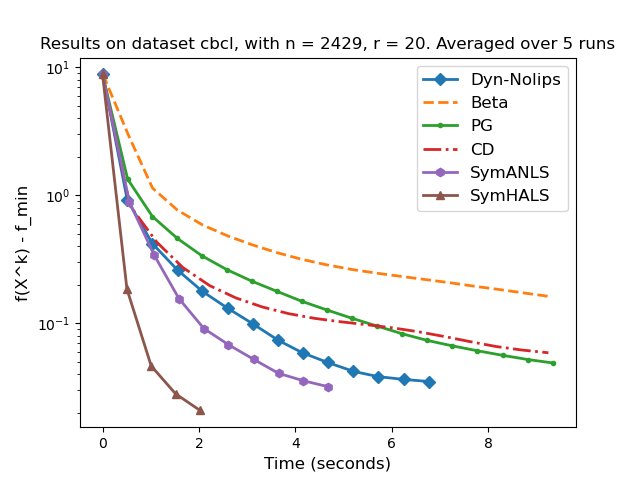
\includegraphics[width=0.8\textwidth]{my_plot_cbcl.png}
    \caption{Зависимость ошибки от времени для CBCL}
    \label{fig:cbcl}
\end{figure}
\begin{table}[h!]
    \centering
    \caption{Данные для CBCL}
    \label{tab:clustering_accuracy_cbcl}
    \begin{tabular}{|l|r|r|r|r|}
        \hline
        Алгоритм & Количество итераций & Время (секунды) & Целевая разность \\
        \hline
        PG & 19 & 9.351 & 0.049 \\
        Dyn-Nolips & 14 & 6.767 & 0.035 \\
        Beta & 19 & 9.288 & 0.162 \\
        CD & 18 & 9.246 & 0.059 \\
        SymHALS & 5 & 2.02 & 0.021 \\
        SymANLS & 10 & 4.686 & 0.032 \\
        \hline
    \end{tabular}
    \end{table}
\newpage

\subsection{Результаты на датасете Coil-20}
\begin{figure}[h!]
    \centering 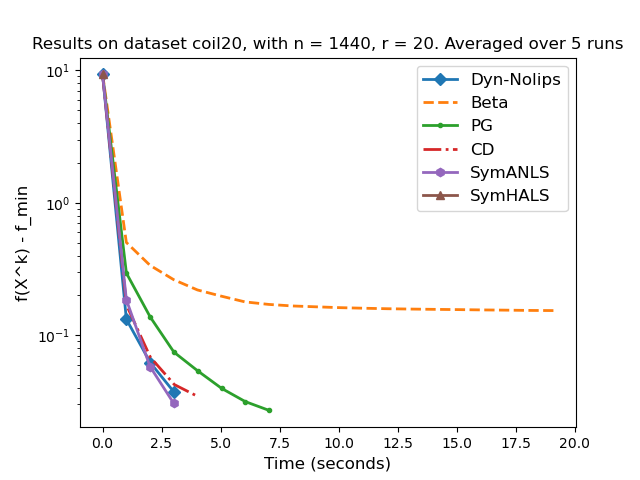
\includegraphics[width=0.8\textwidth]{my_plot_coil20.png}
    \caption{Зависимость ошибки от времени для Coil-20}
    \label{fig:coil20}
\end{figure}
\begin{table}[h!]
    \centering
    \caption{Данные для coil20}
    \label{tab:clustering_accuracy_coil20}
    \begin{tabular}{|l|r|r|r|r|}
        \hline
        Алгоритм & Кластерная точность & Количество итераций & Время (секунды) & Целевая разность \\
        \hline
        PG & 0.717 & 6 & 5.029 & 0.038 \\
        Dyn-Nolips & 0.72 & 4 & 3.026 & 0.037 \\
        Beta & 0.616 & 20 & 19.088 & 0.149 \\
        CD & 0.759 & 5 & 4.062 & 0.028 \\
        SymHALS & 0.492 & 1 & 0.0 & 9.326 \\
        SymANLS & 0.727 & 3 & 2.012 & 0.057 \\
        \hline
    \end{tabular}
    \end{table}
\newpage

\subsection{Результаты на датасете TDT2}
\begin{figure}[h!]
    \centering 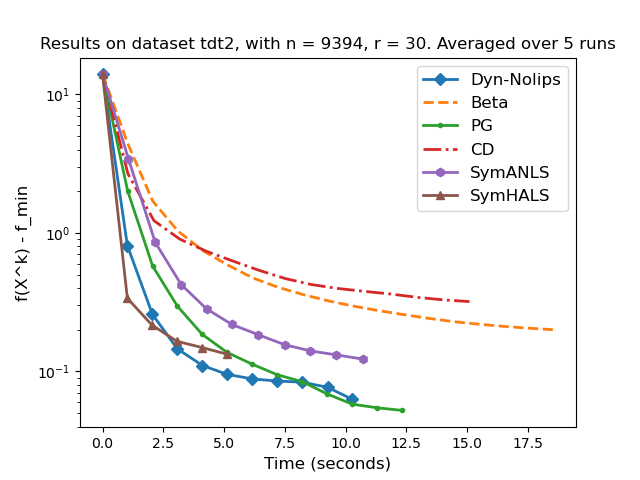
\includegraphics[width=0.8\textwidth]{my_plot_tdt2.png}
    \caption{Зависимость ошибки от времени для TDT2}
    \label{fig:tdt2}
\end{figure}
\begin{table}[h!]
    \centering
    \caption{Данные для TDT2}
    \label{tab:clustering_accuracy_tdt2}
    \begin{tabular}{|l|r|r|r|r|}
        \hline
        Алгоритм & Кластерная точность & Количество итераций & Время (секунды) & Целевая разность \\
        \hline
        PG & 0.849 & 13 & 12.332 & 0.052 \\
        Dyn-Nolips & 0.855 & 11 & 10.284 & 0.063 \\
        Beta & 0.781 & 19 & 18.557 & 0.2 \\
        CD & 0.801 & 15 & 15.102 & 0.319 \\
        SymHALS & 0.841 & 6 & 5.105 & 0.134 \\
        SymANLS & 0.828 & 11 & 10.709 & 0.123 \\
        \hline
    \end{tabular}
\end{table}
\newpage

\subsection{Результаты на датасете Reuters}
\begin{figure}[h!]
    \centering 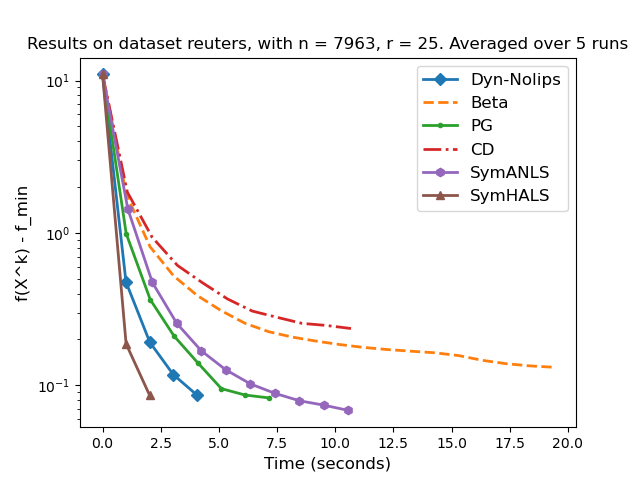
\includegraphics[width=0.8\textwidth]{my_plot_reuters.png}
    \caption{Зависимость ошибки от времени для Reuters}
    \label{fig:reuters}
\end{figure}
\begin{table}[h!]
    \centering
    \caption{Данные для reuters}
    \label{tab:clustering_accuracy_reuters}
    \begin{tabular}{|l|r|r|r|r|}
        \hline
        Алгоритм & Кластерная точность & Количество итераций & Время (секунды) & Целевая разность \\
        \hline
        PG & 0.488 & 19 & 18.507 & 0.078 \\
        Dyn-Nolips & 0.48 & 8 & 7.213 & 0.095 \\
        Beta & 0.383 & 19 & 18.518 & 0.177 \\
        CD & 0.376 & 18 & 18.491 & 0.219 \\
        SymHALS & 0.452 & 3 & 2.037 & 0.11 \\
        SymANLS & 0.486 & 12 & 12.084 & 0.091 \\
        \hline
    \end{tabular}
\end{table}

\section{Заключение}
Dyn-NoLips — это надёжный и универсальный метод, особенно подходящий для больших и разреженных задач, таких как текстовая кластеризация (TDT2, Reuters). Хотя он уступает SymHALS в скорости сходимости, его способность работать без подбора параметров делает его предпочтительным выбором в ситуациях, где требуется высокая автоматизация и устойчивость.

Если точность кластеризации имеет наивысший приоритет, SymANLS может быть предпочтительным выбором, однако это достигается ценой более сложной настройки.

\end{document}

